\providecommand{\hx}{}
\renewcommand{\hx}{\hat{x}}
\providecommand{\hX}{}
\renewcommand{\hX}{\hat{X}}
\providecommand{\hmX}{}
\renewcommand{\hmX}{\hat{\mX}}


\clearpage

\section{Tishby's information bottleneck method}\label{sec:ibmethod}\index{information bottleneck}

\begin{notebox}
\textbf{Paper: } \fullcite{tishbyInformationBottleneckMethod2000}

\hfill Notes taken: 25/12/2019 \index{December 2019}
\end{notebox}


\subsection{Introduction}


In this paper they use information theory, in particular the rate-distortion\index{rate-distortion theory} theory (RDT) of lossy compression, to formulate a problem of encoding a variable (signal) so that the compressed representation contains the \emph{relevant information}\index{relevant information} about some other variable.

\note{Based on \parencite{coverElementsInformationTheory2006}:}
\begin{wrapfigure}{r}{0.3\textwidth}
\vspace{-20pt}
\begin{center}
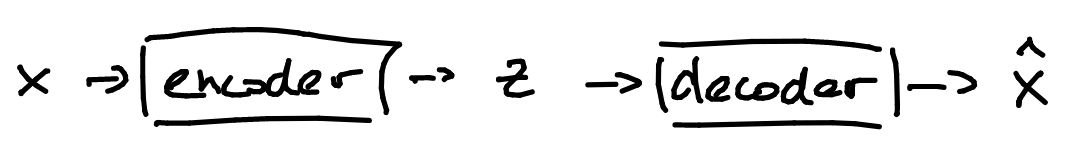
\includegraphics[width=0.3\textwidth]{autoencoder}
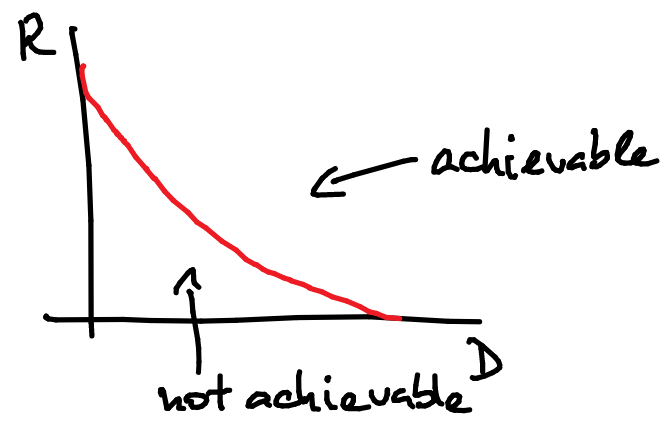
\includegraphics[width=0.25\textwidth]{RDcurve}
\end{center}
\vspace{-20pt}
\caption{\small Rate-distortion encoder and decoder and $R(D)$ curve.}
\vspace{-10pt}
\end{wrapfigure}
In the classical RDT we consider an information source\index{information source} generating sequences of i.i.d. random variables $X$ from \textbf{a known probability distribution} $X \sim p(x)$ with a finite alphabet $X \in \mX$.
We encode the source sequence $x^n \in \mX^n$ through an encoding function $f : \mX^n \to \mZ$ to an index $z \in \mZ = \{1, 2, \ldots, 2^M\}$, where $M$ is the number of bits we can use to represent the source sequence.
The decoder maps the index $z \in \mZ$ to a representation $\hx^n \in \hat{\mX}^n$ of the source sequence $x^n \in \mX^n$ through a decoding function $g : \mZ \to \hat{\mX}^n$. 
The set of possible decodings $\{g(1), g(2), \ldots, g(2^M)\}$ constitutes the \emph{codebook}\index{codebook} and $f^{-1}(z)$ are the \emph{assignment regions}\index{assignment regions}.
Replacement of $X^n$ by $\hX^n$ is commonly referred to as \emph{vector quantization}\index{vector quantization}, representation or reconstruction.

The RDT characterizes the tradeoff between the rate $R = M/n$ (average number of bits per symbol in the source sequence) and the distortion $D = \rE_{p(x)} d(X^n, f\left( g(X^n)\right)$ associated with the code.
The rate-distortion function\index{rate-distortion function} $R(D)$ determines the smallest possible rate for a given distortion $D$.
\note{I think:} If $R = \rH(X)$, this is a lossless autoencoding system where we can achieve zero distortion $D=0$.
With lower rates $R < \rH(X)$ the distortion will increase.

\note{Back to Tishby:}\\
The problem in RDT is that it does not specify which distortion functi~on $d(x, \hx)$ you shall use.\footnote{Classical examples are the squared error loss or Hamming distance.}
Once you pick it, it essentially determines which features of the signal will be considered as \emph{relevant} and encoded into $Z$. 
However, without a definition of \emph{relevance}, this is not a well posed problem. 

What they propose here is to use an additional variable $Y$ to determine what is \emph{relevant} information.
The structure of the problem is then: extract to $\hX$ the info from $X$ that is relevant for predicting $Y$. 
The choice of $Y$ will determine the \emph{relevant features} of the signal. 

\begin{notebox}
\textbf{TLDR:}
Use info theory and rate-distortion theory of encoding $X \to Z \to \hX$ to motivate encoding (compression $\approx$ feature extraction) strategy for classification problem $X \to Z \to \hX \to \hat{Y}$. Careful, $Z \in {1, \ldots, 2^M}$ is an index with $M$ determining the rate of encoding $R = M/n$ ($n$ is the length of the original sequence to be encoded). 
\end{notebox}


\subsection{Relevant quantization}

Assume signal space $\mX$ with fixed \textbf{known prob. distribution $p(x)$} and $\hmX$ its reconstruction space - quantized codebook.
\textbf{Both $\mX$ and $\hmX$ spaces are finite $\approx$ discrete or quantized (if originally continuous).}

For each $x \in \mX$ we seek a possibly \emph{stochastic} mapping to a codeword in the codebook $\hx \in \hmX$ with conditional prob. distribution $\pc{\hx}{x}$.
\begin{equation}
p(\hx) = \sum_x p(x) \pc{\hx}{x} \enspace.
\end{equation}

Average volume of elements of $\mX$ mapped to the same codeword $\hx \in \hmX$ is $2^{\rH(X \mid \hX)}$
\begin{notebox}
This comes from the entropy $\rH(X) = \rE \log_2 1/p(x)$ being the optimal length of encoding. Think of uniform $X$ with $\lvert X \rvert = c$ elements and $p(x) = 1/c$ which has entropy $\rH(X) = 1/c \sum \log_2 c = \log_2 c$.
Then volume is $\lvert X \rvert = c = 2^{\rH(X)}$
\end{notebox}

What matters for the quality of the quantization $\mX$ is a) the average number of bits per codeword $\hX \in \hmX$ and b) the expected distortion between the source and encoding $\rE_{p(x)} d(x, \hx)$. 

The average amount of information (in bits) we gain about $X$ by knowing $\hX$ (or equivalently, the reduction in the average number of bits per element in $X$ knowing $\hX$) is the mutual information
\begin{equation}
\rI(X; \hX) = \sum_{x \in \mX} \sum_{\hx \in \hmX} p(x, \hx) \log \frac{ \pc{\hx}{x} }{p(\hx)} = \rH(\hX) - \rH(\hX \mid X)  = \rH(X) - \rH(X \mid \hX) \enspace .
\end{equation}
For stochastic mappings $\rH(\hX \mid X) \neq 0$ and $\rH(\hX)$ is not what we want to minimize.

\begin{notebox}
\tldr Treat source $\mX$ and reconstruction $\hmX$ spaces as discrete. Allow for stochastic mapping (encoding-decoding) $p(\hx | x)$. Good reconstruction should have high mutual information with the source $\rI(X; \hX) = \sum_{x \in \mX} \sum_{\hx \in \hmX} p(x, \hx) \log \frac{ \pc{\hx}{x} }{p(\hx)}$.
\end{notebox}

\subsection{Relevance through distortion}

The ability to reconstruct is measured in RDT by the distortion function $\mX \times \hmX \to \mR_{+}$ with expected distortion 
\begin{equation}
D = \rE_{p(x, \hx)} d(x, \hx) = \sum_{x \in \mX} \sum_{\hx \in \hmX} d(x, \hx)
\end{equation}
which is presumed to be low for good reconstructions $\hX$ and which implicitly specifies what are the most \emph{relevant} aspects of $X$.

There is a monotonic trade-off between the rate R and the distortion D described by the rate-distortion function $R(D)$\index{rate-distortion function}.
The $R(D)$ function is defined as the minimal achievable rate (mutual information) with a given constraint $D^*$ on the expected distortion
\begin{equation}
R(D) := \min_{\pc{\hx}{x}: \rE_{p(x, \hx)} d(x, \hx) \leq D^*} \rI(X; \hX)
\end{equation}
or in the Lagrangian form as the minimization of 
\begin{equation}
\mL[ \pc{\hx}{x}] = \rI(X; \hX) + \beta \rE_{p(x, \hx)} d(x, \hx) \enspace ,
\end{equation}
where $\beta = -\frac{\dif R}{\dif D} > 0$

For each $\beta$ (that is for each distortion constraint $D^*$) the $\pc{\hx}{x}$ can be found by \emph{Blahut-Arimoto algorithm}\index{Blahut-Arimoto algorithm} which alternates between ensureing that $p(\hx) = \sum_x p(x) \pc{\hx}{x}$ and minimizing the RDT objective.
It's important to note that it only finds the optimal partitioning $\pc{\hx}{x}$ over a given representation space $\hX$.
Finding optimal space $\hX$ would need some sort of EM algorithm.

\begin{notebox}
\tldr In RDT we ere looking for $\pc{\hx}{x}$ which minimizes the mutual information $\rI(X; \hX)$ (minimizes the rate $\approx$ maximizes the compression) with a limit on the expected distortion $\rE_{p(x, \hx)} d(x, \hx) \leq D^*$. This can be formulated as the minimization of 
\begin{equation}
\mL[ \pc{\hx}{x}] = \rI(X; \hX) + \beta \rE_{p(x, \hx)} d(x, \hx) \enspace .
\end{equation}
\end{notebox}

\subsection{Relevance through other variable - information bottleneck}\index{information bottleneck}

As before, we want the quantization $\hX$ to compress $X$ as much as possible but instead of looking at distortion $d(x, \hx)$, we will look at how much information about some third variable $Y$ the quantization $\hX$ can capture $\rI(\hX, Y)$.
We assume that the original signal has positive mutual information with the variable $\rI(X; Y)$ and that the \textbf{true joint distribution $p(x, y)$ is known.}

As lossy compression cannot convey more information than the original data we have $\rI(\hX; Y) \leq \rI(X; Y)$.
The trade-off we look for now is between the rate $\rI(X; \hX)$ (compression) while preserving meaningful info about $Y$: we pass the information $X$ has about $Y$ through a \emph{bottleneck} representation $\hX$.

Similarly to before, we find the optimal $\pc{\hx}{x}$ by minimizing the functional
\begin{equation}
\mL[ \pc{\hx}{x}] = \rI(X; \hX) - \beta \rI(\hX; Y) \enspace ,
\end{equation}
where instead of minimizing the expected distortion $\rE_{p(x, \hx)} d(x, \hx)$ we maximize the mutual information $\rI(\hX; Y)$.

They then proof using the machinery of the Blahut-Arimoto algorithm that the optimal solution is 
\begin{equation}
\pc{\hx}{x} = \frac{p(\hx)}{Z(x, \beta)}
\exp \left[ -\beta \KL{\pc{y}{x}}{\pc{y}{\hx}} \right] \enspace ,
\end{equation}
where $Z(x, \beta)$ is the normalization constant (nothing to do with the encoder $\mZ$.)
This suggest the KL divergence is the \emph{correct} distortion measure in this seeting.
They further propose an algorithm which is alternating between optimizing $\pc{\hx}{x}$, and making sure $p(\hx)$ and $\pc{y}{\hx}$ are consistent with it and the known $p(x, y)$.

\begin{notebox}
\tldr Use some other variable $Y$ with $\rI(X; Y) > 0$ to guide the quality of the representation $\hX$. It should still compress (with low $\rI(X; \hX)$) but instead of $d(x, \hx)$ use $\rI(\hX; Y)$ to see how much the representation preserves from $Y$. The optimization is 
\begin{equation}
\mL[ \pc{\hx}{x}] = \rI(X; \hX) - \beta \rI(\hX; Y) \enspace ,
\end{equation}
and the solution is alternating algo similar to Arimoto-Blahut.
\end{notebox}

\begin{notebox}
\concl 
It is not clear to me what (if anything) can break if we move from the discrete case considered here to the continuous case.
But, more importantly, the assumption that we have access to the true distribution $p(x, y)$ certainly does not hold in ML.
\end{notebox}
